\chapter{Planteamiento del problema}

\section{Diagnóstico}

Los síntomas están en el sector, no en la matriz. En 2018 la migración de plataformas del TSB dejó sin servicio a cerca de 1,9 millones de clientes. Los informes públicos hablan de cientos de millones de libras y de semanas con la operación restringida \cite{UKTreasuryTSB2018}. Ese expediente no nombra OpenAPI ni BIAN. Muestra otra cosa: el negocio y la plataforma se movieron sin una correspondencia que se pudiera verificar.

El \textit{open banking} deja el caso más seco. Desde 2018 la regulación británica obligó a nueve bancos de \textit{retail} a exponer APIs \cite{CMA2016}. Publicar el Swagger no acerca esas interfaces a un modelo de negocio de referencia. Eso se sigue resolviendo en la mesa.

Casas et al.\ \cite{Casas2021} mapearon 47 estudios primarios. Solo el 40\,\% ancla un dominio concreto. El 68\,\% propone herramientas y el 43\,\% mejora la documentación. Golmohammadi et al.\ \cite{Golmohammadi2024}, sobre 92 trabajos de prueba REST, subrayan el costo de validar servicios ya desplegados. Farzi \cite{Farzi2021} acerca BIAN a la agilidad bancaria y deja dicha la distancia entre el \textit{to-be} y lo que corre.

El 21 de noviembre de 2026 buscamos contratos bancarios que se puedan bajar sin cuenta. Aparecen, además de Open Finance Brasil, el Read/Write del Reino Unido (v4.0.1), el XS2A del Berlin Group (v1.3.16) y su openFinance, STET 1.6.3.2, PolishAPI 3.0, el estándar checo 9.0.0, el \textit{Consumer Data Right} australiano (banca 1.36.0), Payments NZ, el marco de Baréin y los YAML de Open Finance de Emiratos en el repositorio de Nebras. Son estándares de cuentas, pagos o ambos. Ninguno trae, en el propio archivo, un score contra un Service Domain BIAN.

\section{Identificación y descripción del problema de estudio}

El objeto no es un banco ni BIAN entero. Es el contrato OpenAPI 3.x con el que el sector describe la API. BIAN entra como modelo de referencia: Service Domains, con behaviors y business objects. La unidad de análisis es la operación del contrato frente al behavior o al objeto del dominio.

En el día a día el desajuste se ve en los nombres. El contrato dice \texttt{paymentRequest} y el dominio dice \texttt{PaymentOrder}. Un PUT del dominio no tiene GET en el YAML, o al revés. En Open Finance Brasil, \texttt{payments} 4.0.0 publica \texttt{POST /pix/payments}. En BIAN v14, Payment Order Initiation llama a esa acción \texttt{Initiate}. \texttt{enrollments} 2.1.0 da de alta un dispositivo (FIDO). No es una orden de pago. Emparejarlo a la fuerza con ese dominio no mide alineación.

BIAN también publica OpenAPI de sus dominios. No por eso medimos BIAN contra BIAN. El archivo que entra es el del estándar o del catálogo: \textit{paths}, \texttt{operationId} y \textit{schemas}. El dominio entra como negocio.

En el sprint, desarrollo publica el YAML. Arquitectura guarda el Service Domain. Un release mueve rutas y el modelo no se entera. La versión del archivo no apunta a una revisión del dominio.

Shabbir et al.\ \cite{Shabbir2025} recuerdan que la consistencia se resiente cuando la documentación técnica no refleja el dominio. La revisión, cuando existe, es una lectura humana o una herramienta genérica de \textit{schema matching} \cite{Shvaiko2005}. No deja el número en el expediente.

\section{Formulación del problema}

\subsection{Formulación del problema general}

Tres capas, y no son la misma frase.

La del sector ya está en el diagnóstico: TSB, los nueve bancos, los YAML públicos. Ahí no hay objeto. Hay síntomas, y el costo que nombran esos informes es retrabajo y adaptadores a ensayo y error.

Si se quita el banco, quedan dos jerarquías. El contrato trae \textit{paths}, operaciones y \textit{schemas}. El Service Domain trae behaviors, business objects y el control. El diagnóstico de esa capa es de correspondencia: el mismo concepto con otro nombre, un verbo que no es el behavior, un esquema que no cubre el objeto, una versión sin rastro.

El problema que la tesis ataca está debajo. Hay lectura humana y hay \textit{schema matching} genérico. No hay un método que, dado un contrato OpenAPI bancario y un Service Domain emparejado, calcule la alineación y la deje repetible. Hoy esa lectura es manual, parcial, o no ocurre antes del despliegue.

\begin{quote}
¿En qué medida y bajo qué tipologías se produce desalineación entre contratos OpenAPI y los modelos de negocio BIAN en arquitecturas API bancarias, y cómo cuantificarla de forma reproducible mediante un modelo de alineación?
\end{quote}

\subsection{Formulación de los problemas específicos}

\begin{enumerate}[label=P\arabic*.]
  \item ¿Qué correspondencias estructurales se pueden armar entre \textit{paths}, operaciones y \textit{schemas} del contrato y los artefactos del Service Domain?
  \item ¿Qué parecido de significado hay entre los nombres del YAML y los conceptos del dominio?
  \item ¿Qué tipologías de desalineación aparecen en un mismo dominio: estructural, semántica, de modelado, de verbo HTTP?
  \item ¿Se pueden juntar esas medidas en un indicador por instancia, el par contrato $\times$ Service Domain?
\end{enumerate}

P1 la responde OE2. P2 la responde OE3. P3 no tiene un cuarto score: las tipologías salen de leer los pares. P4 la responde OE4.

\section{Objetivos}

No hay mediciones previas del grupo. La línea de base son los archivos: el contrato OpenAPI bancario y el Service Domain contra el que se lo lee. El producto de esa línea es la tabla normalizada, S, E, C y el nivel. Tráfico, pruebas y el YAML ya desplegado no entran ahí.

\subsection{Objetivo general}

Diseñar un modelo de alineación que calcule SemanticScore (S), StructuralScore (E), CoverageScore (C) y un AlignmentScore para un contrato OpenAPI bancario frente a un Service Domain BIAN. El prototipo ya calcula ese número. La corrida de todo el corpus contra todos los dominios queda fuera. También queda fuera el YAML de un banco emisor.

El objetivo de más arriba, el del sector, es otro: que un equipo de arquitectura pueda cuantificar esa coherencia antes del despliegue, y bajar el retrabajo de adaptadores y la deriva entre el YAML y el modelo. Esta tesis no implementa ese cambio en un banco. La variable que sí se verifica es el AlignmentScore de cada instancia, en $[0,1]$, con su nivel. S, E y C son el producto de un paso. No reemplazan ese número.

\subsection{Objetivos específicos}

\begin{description}[style=nextline,leftmargin=2.2em]
  \item[OE1.] Normalizar el contrato y el dominio a una fila por operación: ruta, verbo, \texttt{operationId}, esquema y texto.
  \item[OE2.] Emparejar operaciones de forma estructural, uno a uno, y calcular E.
  \item[OE3.] Calcular S sobre esos pares. Hay un S léxico y un S con MiniLM. El segundo no se ajusta con datos nuestros.
  \item[OE4.] Integrar S, E y C en el AlignmentScore y asignar el nivel. Precision, recall, F1 y kappa quedan definidos, y todavía no tienen número.
\end{description}

\begin{table}[H]
  \centering
  \caption{Entrada y salida de cada objetivo}
  \label{tab:oe-io}
  \footnotesize
  \begin{tabular}{@{}p{0.10\textwidth}p{0.40\textwidth}p{0.40\textwidth}@{}}
    \toprule
    ID & Entrada & Salida \\
    \midrule
    OE1 & El contrato y el Service Domain & Una fila por operación: ruta, verbo, \texttt{operationId}, esquema y texto \\
    OE2 & Esas filas & Pares uno a uno, y E en $[0,1]$ \\
    OE3 & Los pares que OE2 congeló & S léxico y S con MiniLM, los dos en $[0,1]$. El oficial es el segundo \\
    OE4 & S, E y las filas de OE1 & C, el AlignmentScore y el nivel \\
    \bottomrule
  \end{tabular}
\end{table}

\section{Metodología}

No hay una hipótesis que contrastar en este borrador. El artefacto es el modelo S, E y C: investigación tecnológica, de diseño. No encuestamos a nadie. Otra persona puede correr el procedimiento. Los números de más abajo ya salieron, y solo de una parte del corpus.

Cinco pasos. Primero se fija el modelo: entradas, S, E, C, la media de los tres y los cortes de nivel. Esos cortes (0,80 / 0,60 / 0,40) son convención de diseño. No salen de etiquetas. Segundo, se adquiere el YAML y se deja en tabla: operación, ruta, verbo, esquema, texto. No armamos grafo ni RDF. Tercero, el greedy estructural. Cuarto, el S, léxico y luego MiniLM, sobre los pares que el tercero congeló. Quinto, C y el AlignmentScore.

El corpus de la tesis son los contratos públicos que el 21 de noviembre se podían bajar sin cuenta (capítulo III, tabla del corpus). El piloto ya parseó 38 YAML de Open Finance Brasil y 258 Service Domains de BIAN v14, 296 de 296. El score no es ese cruce. Es siete instancias. Los estándares en inglés (Reino Unido, Berlin Group, STET, Polonia, Chequia, Australia y los demás de esa tabla) entran al mismo procedimiento. En este borrador todavía no tienen score.

Etiquetamos por separado, match o no-match según el recurso de negocio, no según el verbo. Si no coincidimos, adjudica el asesor. El asesor sigue por designar. Hasta entonces no hay kappa ni F1. I6 quedó en cero. Eso no es nuestra etiqueta.

El despliegue, el \textit{fuzzing} y la latencia no entran. Tampoco usamos el contrato como entrada de una prueba \cite{Ehsan2022,Golmohammadi2024}. FDX existe para Estados Unidos y Canadá, y el YAML no se baja sin registro.

\section{Objeto de estudio}

El objeto no es un banco ni BIAN entero. Son los contratos OpenAPI con los que el sector describe sus APIs. Quedan fuera del objeto la organización BIAN, el código de los backends y la infraestructura. BIAN entra como modelo de referencia.

\begin{figure}[H]
  \centering
  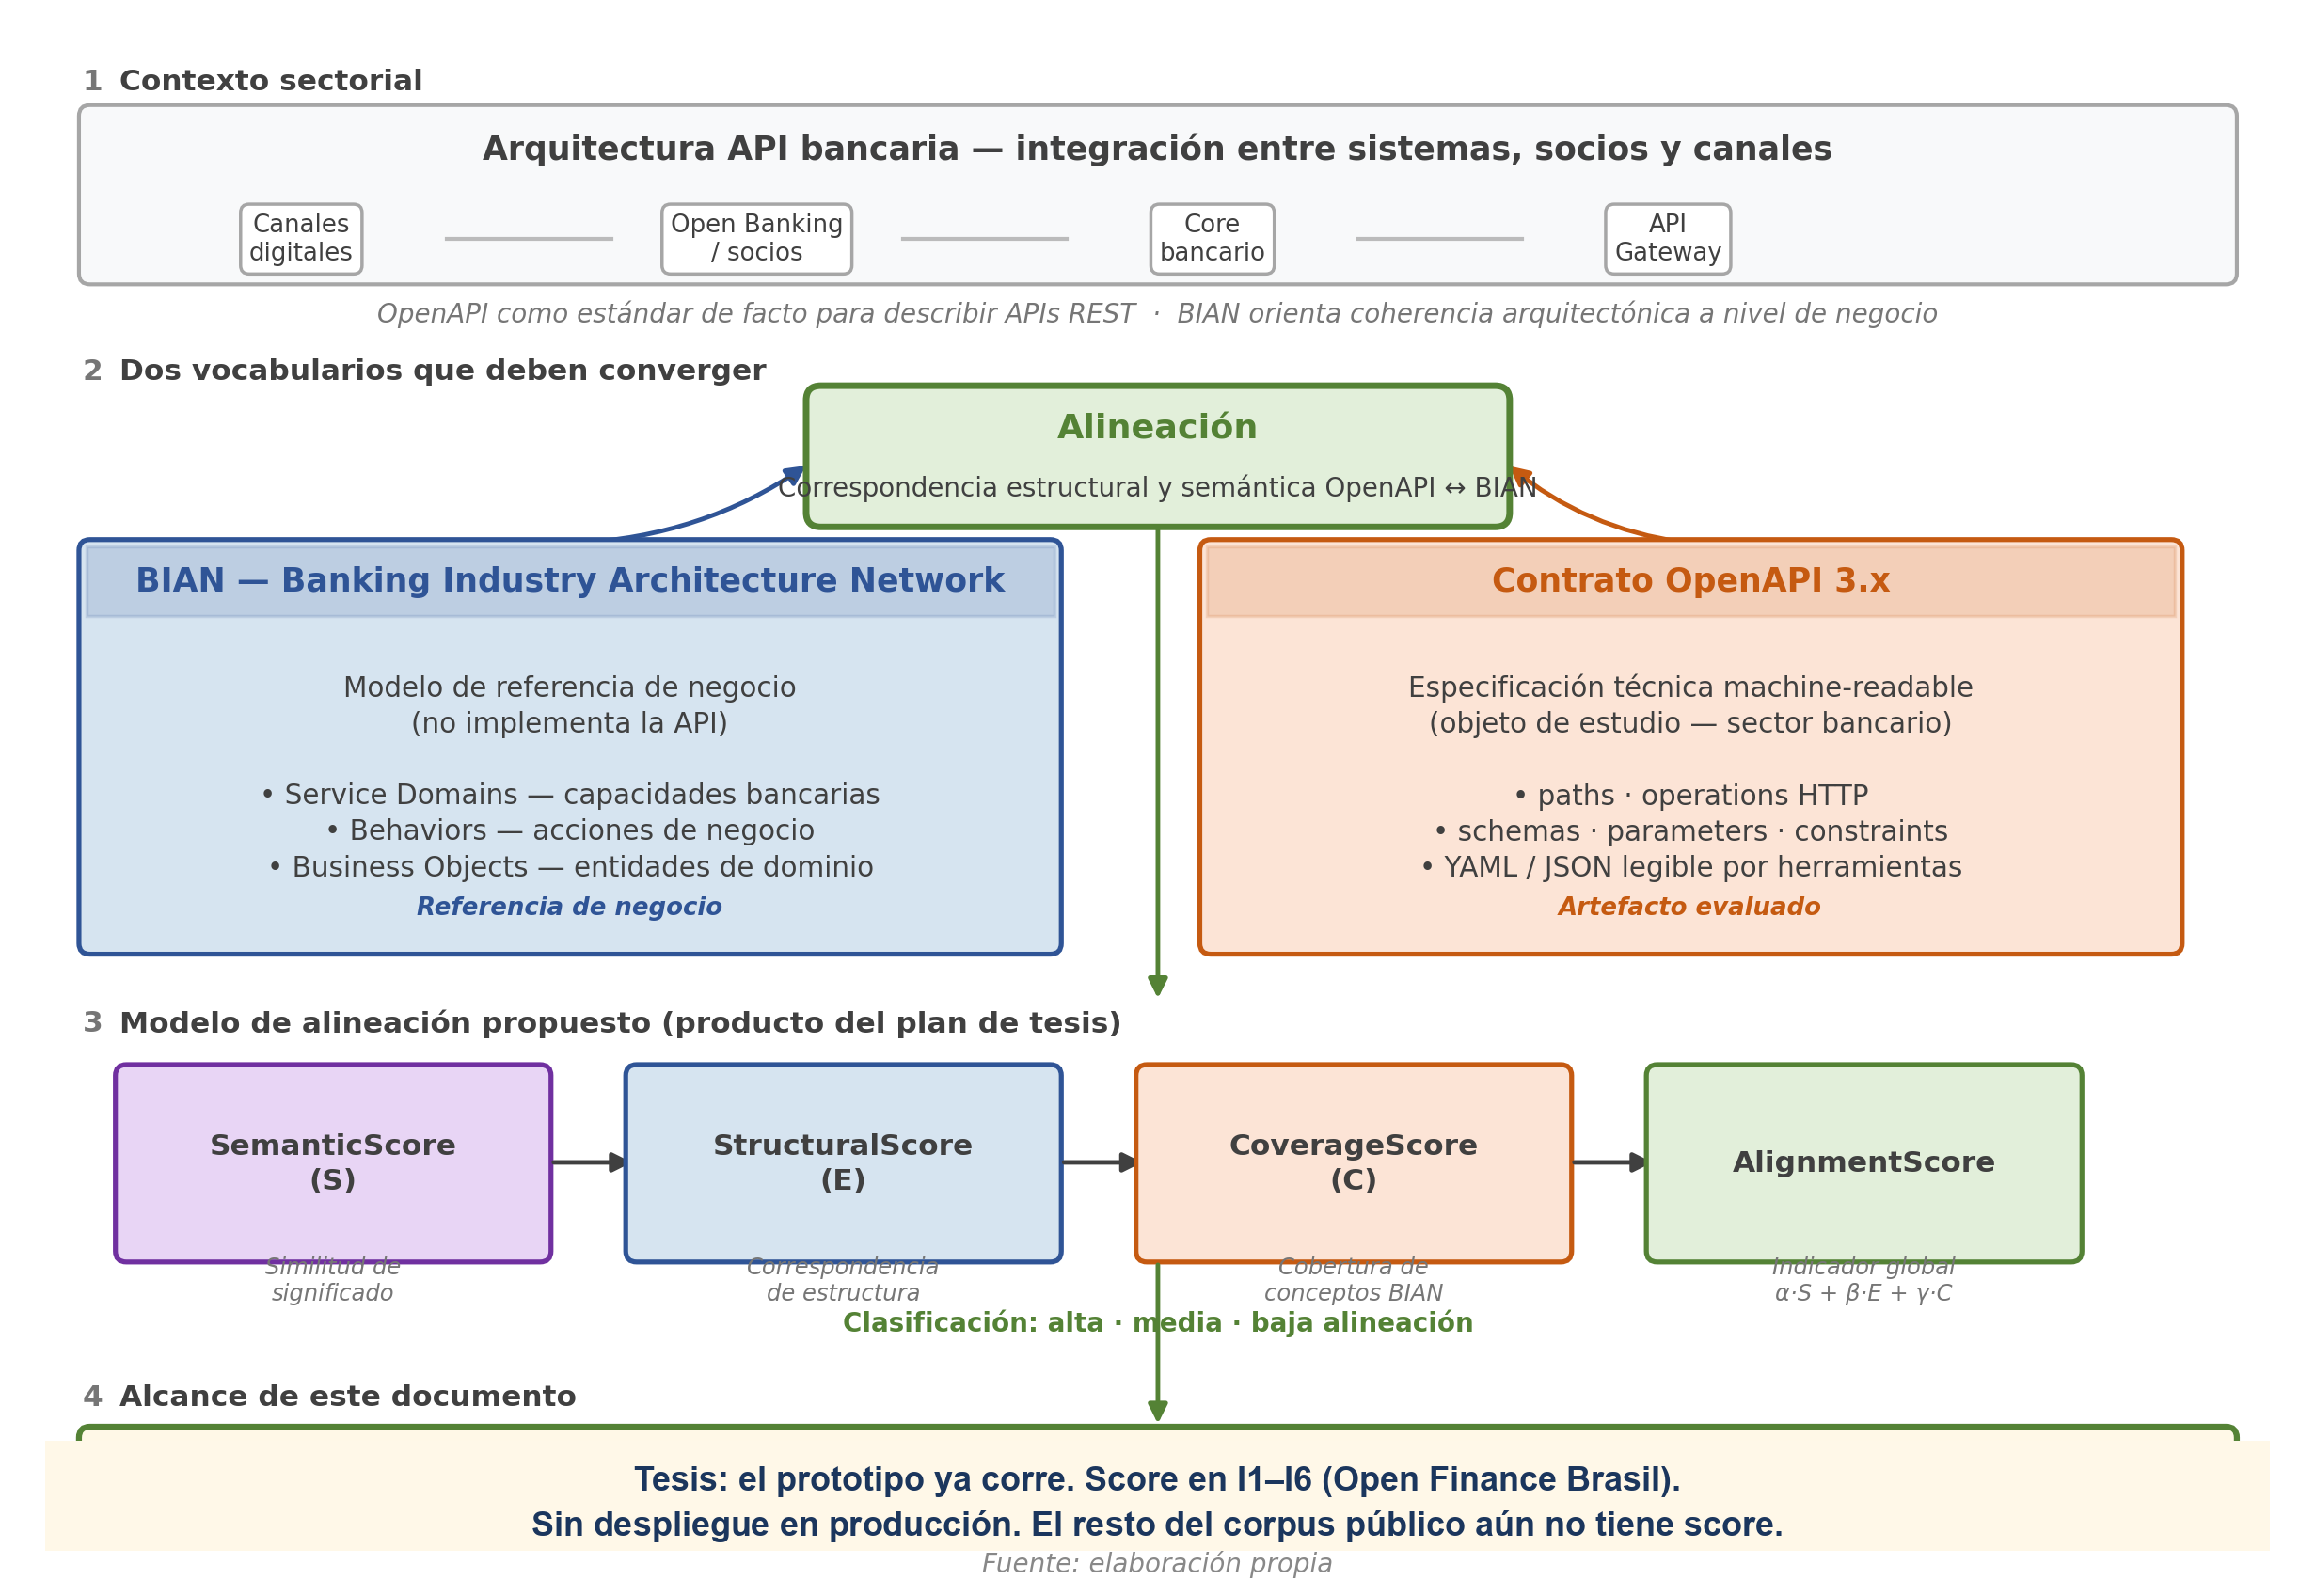
\includegraphics[width=0.92\textwidth]{Figura_01_Contexto}
  \caption{Contexto: arquitectura API bancaria, BIAN, OpenAPI y modelo S/E/C}
  \label{fig:contexto}
\end{figure}

\begin{figure}[H]
  \centering
  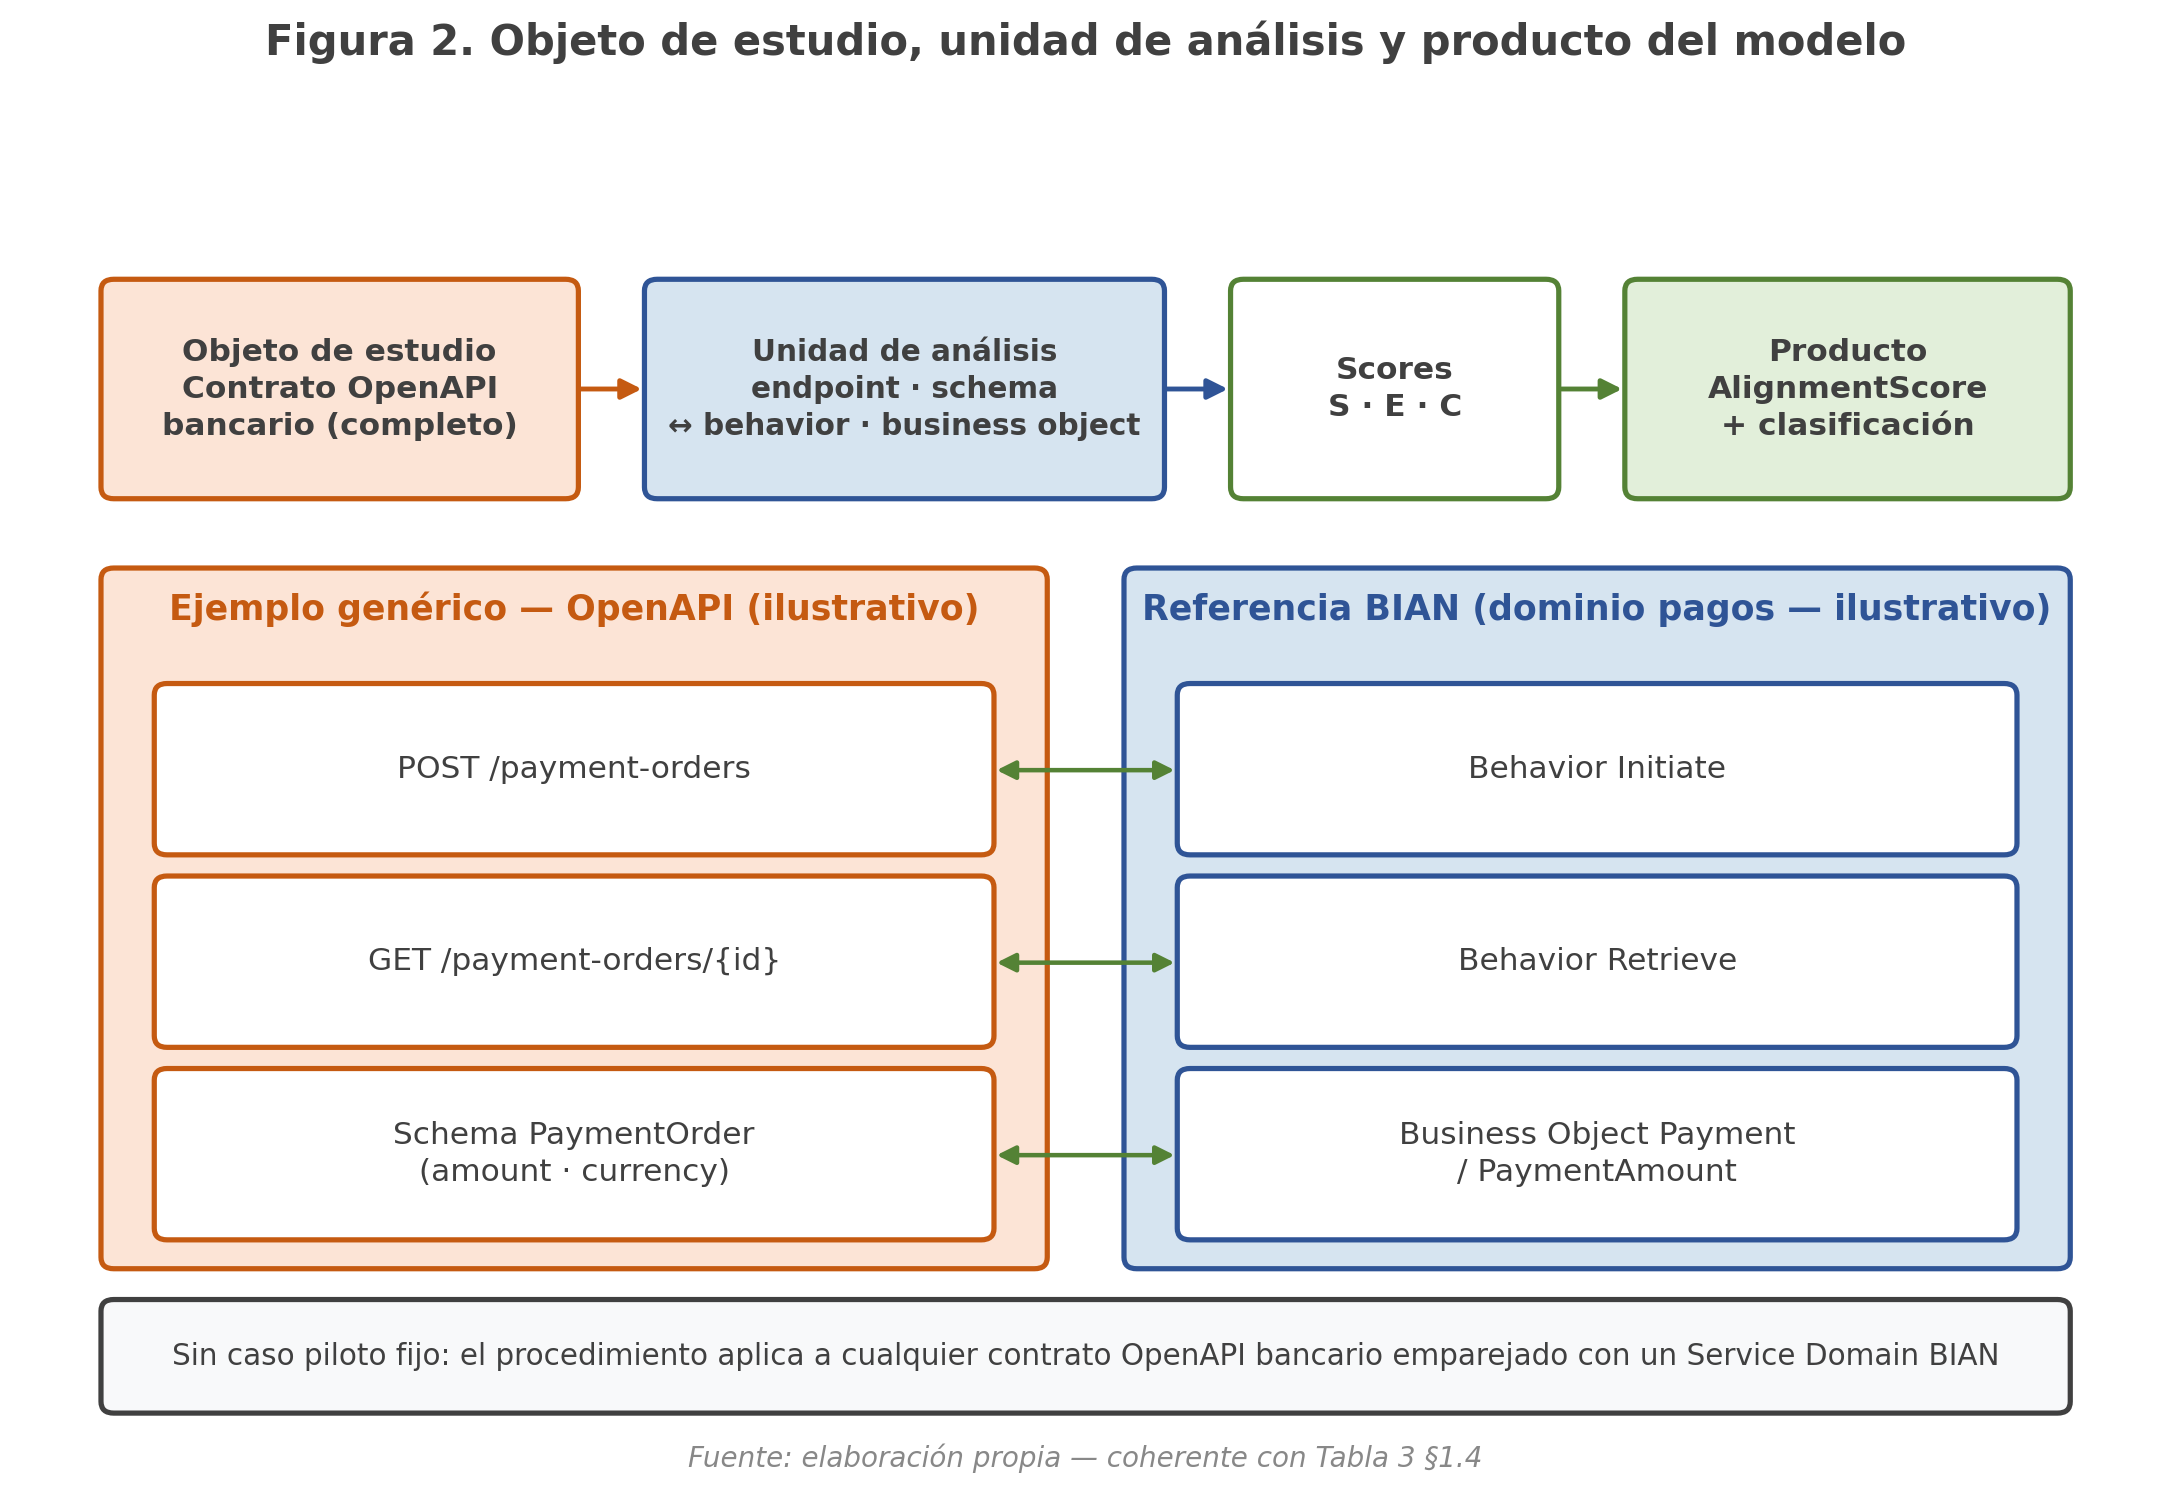
\includegraphics[width=0.88\textwidth]{Figura_02_Objeto_Unidad_Analisis}
  \caption{Objeto, referencia BIAN, unidad de análisis y producto del modelo}
  \label{fig:objeto}
\end{figure}

\begin{table}[H]
  \centering
  \caption{Objeto, unidad de análisis y producto}
  \label{tab:objeto}
  \begin{tabular}{@{}p{0.28\textwidth}p{0.62\textwidth}@{}}
    \toprule
    Concepto & En este estudio \\
    \midrule
    Objeto de estudio & El contrato OpenAPI bancario (el archivo) \\
    Unidad de análisis & Operación o esquema del contrato frente a un behavior o business object del Service Domain \\
    Producto & S, E, C y AlignmentScore por instancia contrato $\times$ dominio \\
    \bottomrule
  \end{tabular}
\end{table}

Cada instancia se nombra con la fuente, el dominio y la versión. I1 es \texttt{accounts} 2.4.2 contra Savings Account. El corpus público del capítulo III amplía las fuentes. No cambia el objeto.

\begin{table}[H]
  \centering
  \caption{Tipología de desalineaciones}
  \label{tab:tipologias}
  \small
  \begin{tabular}{@{}p{0.18\textwidth}p{0.38\textwidth}p{0.34\textwidth}@{}}
    \toprule
    Tipo & Qué es & Ejemplo \\
    \midrule
    Estructural & La organización de endpoints no sigue la del dominio & \texttt{POST /transfer} sin el behavior \texttt{Initiate} \\
    Semántica & La estructura se parece y el negocio no & \texttt{amount} sin vínculo con \texttt{PaymentAmount} \\
    De modelado & Falta una entidad o un atributo obligatorio & Un esquema que omite campos del business object \\
    REST / contrato & El verbo o la ruta no se leen como operación de negocio & Un verbo metido en la URL \\
    \bottomrule
  \end{tabular}
\end{table}

\section{Ámbito y delimitación}

El ámbito es el archivo público, no el banco. La tabla fija sector, artefactos, técnica, geografía y tiempo. Quedan fuera el despliegue, las pruebas de penetración y medir latencia en ejecución.

\begin{table}[H]
  \centering
  \caption{Ámbito del estudio}
  \label{tab:ambito}
  \begin{tabular}{@{}p{0.24\textwidth}p{0.66\textwidth}@{}}
    \toprule
    Dimensión & Delimitación \\
    \midrule
    Sector & Banca y servicios financieros con APIs \\
    Artefactos & Contratos OpenAPI o Swagger públicos, y Service Domains BIAN v14 \\
    Técnica & Análisis estructural y similitud semántica \\
    Geografía & No restringida. Los casos son documentación pública \\
    Tiempo & Especificaciones vigentes en 2024--2026. La lista de corpus se cerró el 21 de noviembre de 2026 \\
    \bottomrule
  \end{tabular}
\end{table}

\section{Alcances y limitaciones}
\label{sec:alcances}

El modelo ya está en un prototipo, y el piloto de siete instancias ya tiene número. La tabla separa eso de lo que sigue fuera: el YAML de un banco emisor, la corrida de todo el corpus contra los 258 dominios, y el despliegue. Los demás estándares públicos entran al corpus y, en este borrador, no tienen score.

\begin{table}[H]
  \centering
  \caption{Alcances y limitaciones}
  \label{tab:alcances}
  \footnotesize
  \begin{tabular}{@{}p{0.46\textwidth}p{0.46\textwidth}@{}}
    \toprule
    Alcance & Limitación \\
    \midrule
    Medir alineación estructural y semántica entre un contrato OpenAPI y un Service Domain & No desplegar APIs \\
    Dejar métricas que otra persona pueda repetir & No sustituir una certificación ni una auditoría legal \\
    El modelo S, E, C y el AlignmentScore & No puntuar los 258 dominios contra todo el corpus \\
    El corpus de contratos públicos del capítulo III & FDX y los PDF sin YAML no entran al parser \\
    El prototipo y el piloto de siete instancias, ya corrido & El resto del corpus todavía no tiene score \\
    Niveles Alta, Media, Baja y Nula & Los cortes son convención. No hay F1 \\
    \bottomrule
  \end{tabular}
\end{table}

\section{Justificación}

Si un release mueve el YAML y el Service Domain se queda en el modelo, el desfase se ve en el archivo: un path nuevo, un \texttt{operationId} que ya no nombra el behavior, un \texttt{\$ref} que apunta a otro esquema. Farzi \cite{Farzi2021} y Bhatia \cite{Bhatia2022} describen esa deriva entre producto, integración y gobernanza cuando el contrato y BIAN no se rastrean. Conviene verla en el archivo, no cuando el servicio ya está en producción.

Revisar a mano no escala cuando hay decenas de APIs y de socios. El AlignmentScore ordena esa cola con un número \cite{Shabbir2025}. OpenAPI, como artefacto, ya está maduro \cite{Casas2021}. Lo que no teníamos escrito es el cruce con un Service Domain. El procedimiento de esta tesis es esa pieza.

La pregunta cabe en el archivo. Este contrato, en esta versión, ¿refleja este Service Domain? S y E salen de ahí. No son una prueba en ejecución, ni un sello.

\section{Clasificación IEEE / ACM}

El tema cae en representación de conocimiento y en redes semánticas. No es testing de APIs ni un clasificador entrenado con nuestros pares.

\begin{table}[H]
  \centering
  \caption{Clasificación IEEE / ACM}
  \label{tab:clasificacion}
  \begin{tabular}{@{}p{0.16\textwidth}p{0.28\textwidth}p{0.46\textwidth}@{}}
    \toprule
    Taxonomía & Categoría & Por qué \\
    \midrule
    IEEE & Knowledge Representation &
    El contrato y el Service Domain son dos representaciones del mismo negocio. Medimos si se corresponden \\
    ACM & Semantic networks &
    El emparejamiento y la similitud entre conceptos de negocio y piezas de la API caen en redes de significado y en alineación de esquemas \\
    \bottomrule
  \end{tabular}
\end{table}

\section{Hipótesis de trabajo}

No las contrastamos en este borrador. Cada una nombra el producto de un objetivo y el ratio que se mediría cuando haya etiquetas.

\begin{enumerate}
  \item H1, ligada a OE1. Normalizar el contrato y el dominio en la misma tabla permite calcular S, E y C. El ratio es la completitud de la extracción.
  \item H2, ligada a OE2. El schema matching de Shvaiko y Euzenat \cite{Shvaiko2005} produce un StructuralScore de la correspondencia REST--dominio.
  \item H3, ligada a OE3. La similitud semántica \cite{ElBayadh2015,Chandrasekaran2022} produce un SemanticScore que separa un concepto alineado de uno que no lo está.
  \item H4, ligada a OE4. La media de S, E y C produce un AlignmentScore que se puede clasificar por nivel.
\end{enumerate}

\section{Factores y ratios}

Los factores son decisiones de diseño. Los ratios son los números. En esta corrida los factores ya están elegidos: tabla y no grafo, greedy con los pesos 0,40 / 0,25 / 0,20 / 0,15, S léxico y MiniLM, pesos iguales en el score oficial.

\begin{table}[H]
  \centering
  \caption{Factores y ratios}
  \label{tab:variables}
  \footnotesize
  \begin{tabular}{@{}p{0.12\textwidth}p{0.28\textwidth}p{0.24\textwidth}p{0.26\textwidth}@{}}
    \toprule
    Pieza & Factor & Ratio & Control \\
    \midrule
    OG & Pesos del AlignmentScore & Score y nivel & $\alpha+\beta+\gamma=1$. Cortes fijos \\
    OE1 & Representación intermedia & Extraídos / esperados & Versión fija del YAML y del dominio \\
    OE2 & Regla de matching & E en $[0,1]$ & Mismos pares normalizados \\
    OE3 & Encoder & S en $[0,1]$ & Mismos pares. Sin fine-tuning \\
    OE4 & Pesos & C, y el score global & Los tres pesos suman 1 \\
    \bottomrule
  \end{tabular}
\end{table}

\begin{figure}[H]
  \centering
  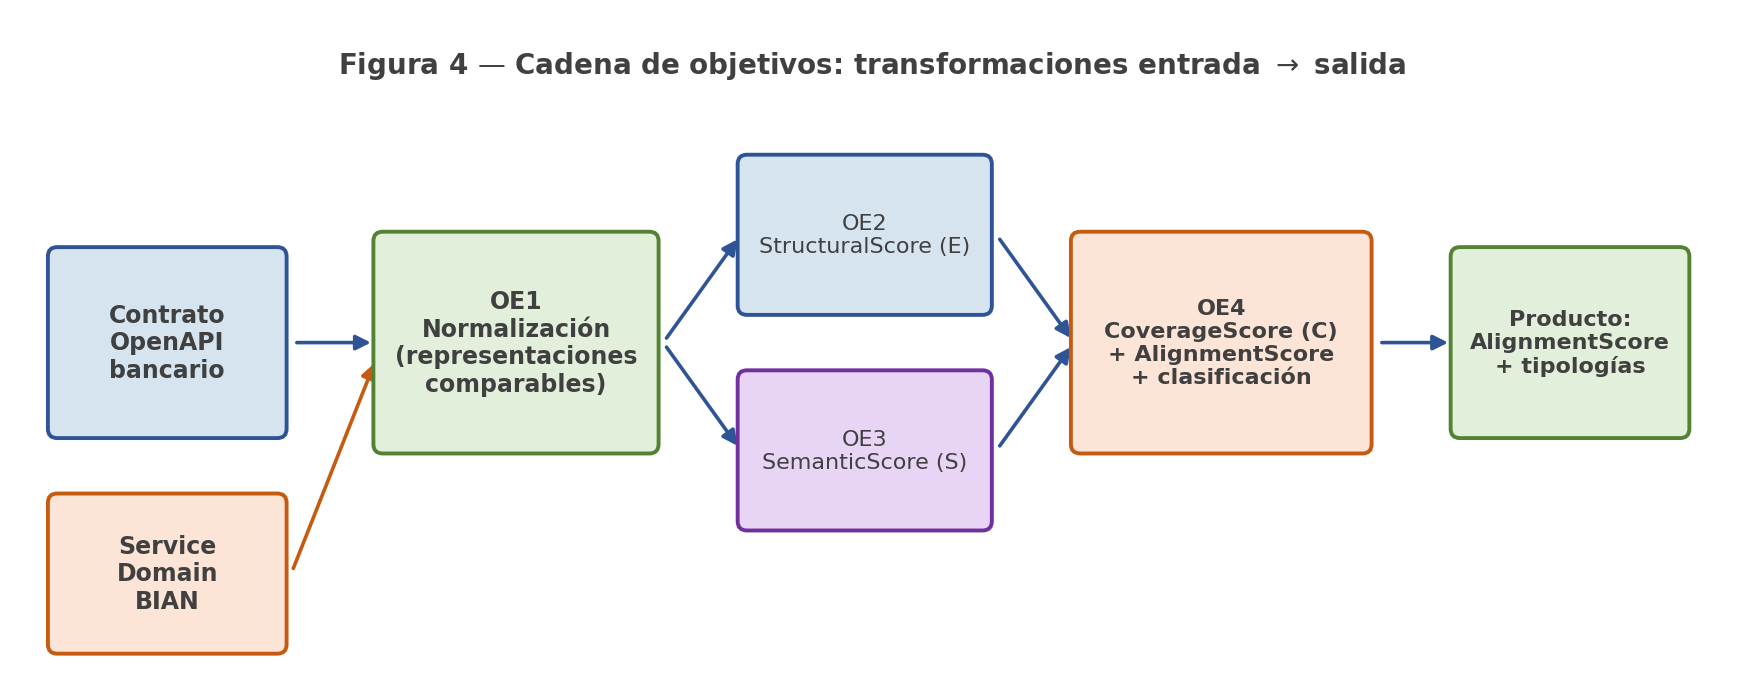
\includegraphics[width=0.98\textwidth]{Figura_04_Cadena_Objetivos}
  \caption{Cadena: normalizar, calcular S, E y C, integrar el AlignmentScore}
  \label{fig:cadena}
\end{figure}

